\documentclass[12pt]{article}
\usepackage[margin=1in]{geometry}
\usepackage{amsmath,amsfonts,amssymb}
\usepackage{graphicx}
\usepackage{booktabs}
\usepackage{longtable}
\usepackage{pdflscape}
\usepackage{rotating}
\usepackage{caption}
\usepackage{subcaption}
\usepackage{setspace}
\usepackage{hyperref}
\usepackage{float}
\usepackage{array}
\usepackage{multirow}
\usepackage{threeparttable}
\usepackage{rotating}
\usepackage{comment}
\usepackage[backend=biber, style=authoryear, natbib]{biblatex}
\usepackage{booktabs}
\usepackage{setspace}
\addbibresource{casino.bib} 
\renewcommand*{\nameyeardelim}{\addcomma\addspace}

% Custom commands for better table formatting
\newcommand{\specialcell}[2][c]{%
  \begin{tabular}[#1]{@{}c@{}}#2\end{tabular}}

\title{The Destruction of Social Capital and Family Flight: Evidence from Casino Openings}
\author{Malcolm Kass\thanks{University of Dallas, Department of Economics. Email: mkass@udallas.edu} \and John Soriano\thanks{University of Dallas, Department of Economics. Email: jsoriano@udallas.edu}}
\date{\today}

\begin{document}

\maketitle

\begin{abstract}
Casino development is often promoted as an engine of local economic growth, but its broader social consequences remain less understood. This paper investigates how casino openings reshape demographic patterns and family-supporting institutions in U.S. counties from 2003 to 2023. Exploiting staggered treatment timing in a difference-in-differences framework, we document consistent evidence that casinos erode community structures. We estimate a 1.28 percentage point decline in fertility rates for women, tied to an estimated drop of 55 children per 1000 women and 26 children per 1000 men. These effects are not a result of new movers to the community where a new casino opened. These demographic shifts are mirrored in weakened religious institutions: religious adherence declines by an estimated 9.5 percentage points, particularly in Catholic communities. The results demonstrate that casinos generate possible social capital losses alongside their economic activity, altering the composition of local populations and undermining religious institutions historically central to family and community life.
\end{abstract}

\begin{comment}
This paper examines the effects of casino openings on family formation and community institutions using a differences-in-differences design with staggered casino openings across U.S. counties from 2000-2023. We find that casinos systematically reduce fertility and disrupt family-supporting institutions through both behavioral change among long-term residents and selective migration. Population declines are concentrated among children and child-rearing age adults, while religious adherence and school enrollment also decline significantly.
\end{comment}
\newpage

\section{Introduction}

Table \ref{tab:summary} 

% Table 1: Summary Statistics - Input directly without wrapper
\begin{table}[htbp]\centering
\def\sym#1{\ifmmode^{#1}\else\(^{#1}\)\fi}
\caption{Summary Statistics by County Type}
\label{tab:summary}
\begin{tabular}{l*{3}{cc}}
\hline\hline
            &\multicolumn{2}{c}{(1)}  &\multicolumn{2}{c}{(2)}  &\multicolumn{2}{c}{(3)}  \\
            &\multicolumn{2}{c}{Casino Counties}&\multicolumn{2}{c}{Nearby Counties}&\multicolumn{2}{c}{Control Counties}\\
            &        mean&          sd&        mean&          sd&        mean&          sd\\
\hline
married     &       0.313&       0.464&       0.343&       0.475&       0.379&       0.485\\
has\_children&       0.347&       0.476&       0.368&       0.482&       0.409&       0.492\\
num\_children&       0.701&       1.142&       0.740&       1.153&       0.823&       1.186\\
female      &       0.496&       0.500&       0.495&       0.500&       0.495&       0.500\\
age         &      29.086&       6.558&      29.031&       6.636&      29.042&       6.685\\
white       &       0.575&       0.494&       0.666&       0.472&       0.707&       0.455\\
black       &       0.157&       0.364&       0.120&       0.325&       0.131&       0.338\\
hispanic    &       0.287&       0.452&       0.209&       0.407&       0.178&       0.382\\
\hline
\(N\)       &     3305201&            &     2491622&            &    16503448&            \\
\hline\hline
\multicolumn{7}{l}{\footnotesize Notes: Individual-level statistics weighted by person weights. Sample includes individuals aged 18-40.}\\
\end{tabular}
\end{table}


\section{Population Effects}
We begin by documenting population effects across age groups. Table \ref{tab:population} 

% Table 2: Population Effects - Input directly without wrapper
\begin{table}[htbp]\centering
\def\sym#1{\ifmmode^{#1}\else\(^{#1}\)\fi}
\caption{Population Effects by Age Group}
\begin{tabular}{l*{4}{c}}
\hline\hline
            &\multicolumn{1}{c}{Total Pop}&\multicolumn{1}{c}{Child-Rearing}&\multicolumn{1}{c}{Children}&\multicolumn{1}{c}{School-Age}\\\cmidrule(lr){2-2}\cmidrule(lr){3-3}\cmidrule(lr){4-4}\cmidrule(lr){5-5}
            &\multicolumn{1}{c}{(1)}&\multicolumn{1}{c}{(2)}&\multicolumn{1}{c}{(3)}&\multicolumn{1}{c}{(4)}\\
            &\multicolumn{1}{c}{ln\_total\_pop}&\multicolumn{1}{c}{ln\_child\_rearing\_pop}&\multicolumn{1}{c}{ln\_children\_pop}&\multicolumn{1}{c}{ln\_school\_age\_pop}\\
\hline
t-3         &      -0.042\sym{**} &      -0.032\sym{*}  &      -0.055\sym{***}&      -0.059\sym{***}\\
            &     (0.017)         &     (0.018)         &     (0.021)         &     (0.022)         \\
[1em]
t-2         &       0.010\sym{*}  &       0.002         &       0.015         &       0.017\sym{*}  \\
            &     (0.006)         &     (0.013)         &     (0.009)         &     (0.010)         \\
[1em]
t           &       0.002         &      -0.005         &      -0.009         &      -0.009         \\
            &     (0.006)         &     (0.012)         &     (0.009)         &     (0.009)         \\
[1em]
t+1         &      -0.011         &      -0.015         &      -0.014         &      -0.014         \\
            &     (0.009)         &     (0.015)         &     (0.012)         &     (0.012)         \\
[1em]
t+2         &      -0.021\sym{**} &      -0.011         &      -0.026\sym{*}  &      -0.025\sym{*}  \\
            &     (0.009)         &     (0.013)         &     (0.013)         &     (0.014)         \\
[1em]
t+3         &      -0.023\sym{**} &      -0.003         &      -0.027\sym{*}  &      -0.033\sym{**} \\
            &     (0.012)         &     (0.017)         &     (0.016)         &     (0.016)         \\
[1em]
t+4         &      -0.026\sym{**} &      -0.009         &      -0.033\sym{**} &      -0.038\sym{**} \\
            &     (0.013)         &     (0.017)         &     (0.017)         &     (0.017)         \\
[1em]
t+5         &      -0.029\sym{**} &      -0.017         &      -0.039\sym{**} &      -0.043\sym{**} \\
            &     (0.013)         &     (0.019)         &     (0.017)         &     (0.018)         \\
[1em]
t+6         &      -0.031\sym{**} &      -0.016         &      -0.047\sym{**} &      -0.051\sym{**} \\
            &     (0.015)         &     (0.021)         &     (0.019)         &     (0.020)         \\
[1em]
t+7         &      -0.038\sym{**} &      -0.019         &      -0.050\sym{**} &      -0.052\sym{**} \\
            &     (0.015)         &     (0.021)         &     (0.020)         &     (0.021)         \\
[1em]
t+8+        &      -0.030         &      -0.003         &      -0.040\sym{*}  &      -0.046\sym{*}  \\
            &     (0.020)         &     (0.024)         &     (0.024)         &     (0.026)         \\
\hline
Observations&       6,686         &       6,686         &       6,686         &       6,686         \\
R-squared   &       0.993         &       0.991         &       0.992         &       0.991         \\
\hline\hline
\multicolumn{5}{l}{\footnotesize Standard errors in parentheses}\\
\multicolumn{5}{l}{\footnotesize Standard errors clustered at county level in parentheses.}\\
\multicolumn{5}{l}{\footnotesize Donut sample excludes nearby counties. All variables in logs.}\\
\multicolumn{5}{l}{\footnotesize \sym{*} \(p<0.10\), \sym{**} \(p<0.05\), \sym{***} \(p<0.01\)}\\
\end{tabular}
\end{table}


Figure \ref{fig:population} 

\begin{figure}[H]
\centering
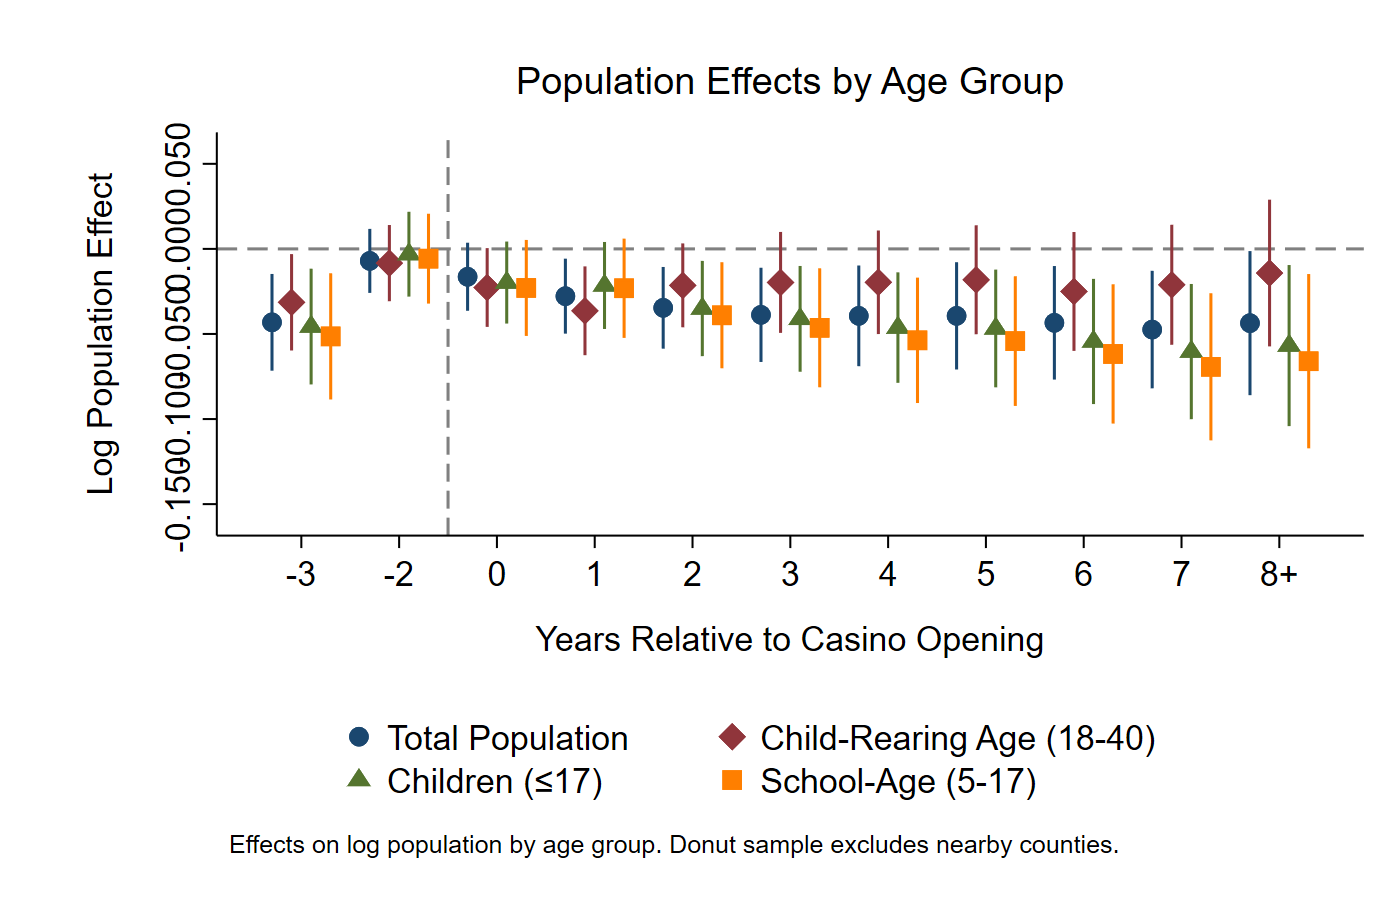
\includegraphics[width=\textwidth]{figure1_population_effects.png}
\caption{Population Effects by Age Group}
\label{fig:population}
\end{figure}
 Table \ref{tab:family} presents difference-in-differences results for marriage, childbearing, and fertility by gender.

% Table 3: Family Formation Effects - Input directly without wrapper
\begin{table}[htbp]\centering
\def\sym#1{\ifmmode^{#1}\else\(^{#1}\)\fi}
\caption{Family Formation Effects by Gender}
\begin{tabular}{l*{6}{c}}
\hline\hline
            &\multicolumn{3}{c}{Women}                                        &\multicolumn{3}{c}{Men}                                          \\\cmidrule(lr){2-4}\cmidrule(lr){5-7}
            &\multicolumn{1}{c}{(1)}&\multicolumn{1}{c}{(2)}&\multicolumn{1}{c}{(3)}&\multicolumn{1}{c}{(4)}&\multicolumn{1}{c}{(5)}&\multicolumn{1}{c}{(6)}\\
            &\multicolumn{1}{c}{Marriage}&\multicolumn{1}{c}{Has Children}&\multicolumn{1}{c}{Num Children}&\multicolumn{1}{c}{Marriage}&\multicolumn{1}{c}{Has Children}&\multicolumn{1}{c}{Num Children}\\
\hline
post\_treatment&     -0.0006         &     -0.0098\sym{***}&     -0.0375\sym{***}&      0.0009         &     -0.0057         &     -0.0251\sym{***}\\
            &    (0.0055)         &    (0.0030)         &    (0.0073)         &    (0.0032)         &    (0.0048)         &    (0.0087)         \\
\hline
Observations&   7,543,963         &   7,543,963         &   7,543,963         &   7,638,910         &   7,638,910         &   7,638,910         \\
R-squared   &       0.206         &       0.270         &       0.241         &       0.219         &       0.227         &       0.204         \\
\hline\hline
\multicolumn{7}{l}{\footnotesize Standard errors in parentheses}\\
\multicolumn{7}{l}{\footnotesize Standard errors clustered at county level in parentheses.}\\
\multicolumn{7}{l}{\footnotesize All regressions include county and year fixed effects, age and age squared.}\\
\multicolumn{7}{l}{\footnotesize Donut sample excludes nearby counties. *** p<0.01, ** p<0.05, * p<0.1.}\\
\multicolumn{7}{l}{\footnotesize \sym{*} \(p<0.10\), \sym{**} \(p<0.05\), \sym{***} \(p<0.01\)}\\
\end{tabular}
\end{table}

 Figure \ref{fig:fertility} shows these fertility effects emerge immediately after casino opening and persist throughout our observation window.

\begin{figure}[H]
\centering
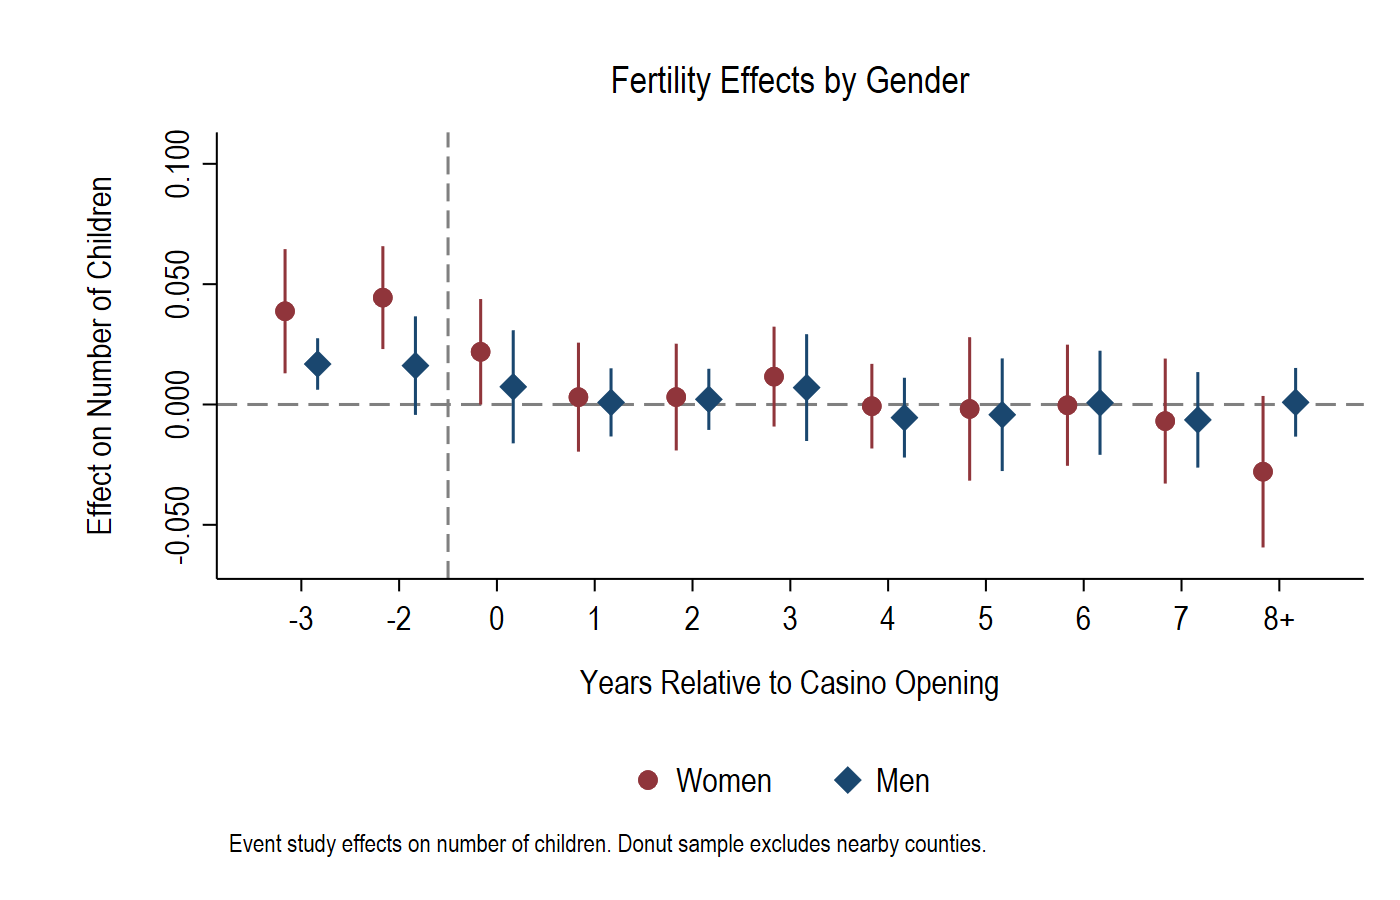
\includegraphics[width=\textwidth]{figure2_fertility_effects.png}
\caption{Fertility Effects by Gender}
\label{fig:fertility}
\end{figure}


Table \ref{tab:mechanism} 

% Table 4: Effects by Residence Duration - Input directly without wrapper
\begin{table}[htbp]\centering
\def\sym#1{\ifmmode^{#1}\else\(^{#1}\)\fi}
\caption{Effects by Residence Duration: Number of Children}
\begin{tabular}{l*{4}{c}}
\hline\hline
            &\multicolumn{2}{c}{Women}                  &\multicolumn{2}{c}{Men}                    \\\cmidrule(lr){2-3}\cmidrule(lr){4-5}
            &\multicolumn{1}{c}{(1)}&\multicolumn{1}{c}{(2)}&\multicolumn{1}{c}{(3)}&\multicolumn{1}{c}{(4)}\\
            &\multicolumn{1}{c}{Long-term (5+)}&\multicolumn{1}{c}{Recent (<5)}&\multicolumn{1}{c}{Long-term (5+)}&\multicolumn{1}{c}{Recent (<5)}\\
\hline
-3          &       0.016         &      -0.048\sym{**} &       0.051         &      -0.010         \\
            &     (0.068)         &     (0.021)         &     (0.040)         &     (0.017)         \\
[1em]
-2          &       0.027         &       0.035         &      -0.025         &       0.009         \\
            &     (0.044)         &     (0.034)         &     (0.026)         &     (0.028)         \\
[1em]
0           &      -0.003         &      -0.035         &       0.032         &      -0.034         \\
            &     (0.052)         &     (0.023)         &     (0.055)         &     (0.023)         \\
[1em]
1           &       0.035         &      -0.047\sym{*}  &      -0.038         &      -0.040\sym{***}\\
            &     (0.069)         &     (0.024)         &     (0.053)         &     (0.014)         \\
[1em]
2           &      -0.014         &       0.000         &      -0.025         &      -0.013         \\
            &     (0.050)         &     (0.028)         &     (0.036)         &     (0.014)         \\
[1em]
3           &       0.045         &      -0.013         &      -0.007         &      -0.007         \\
            &     (0.043)         &     (0.019)         &     (0.055)         &     (0.021)         \\
[1em]
4           &       0.022         &      -0.032         &      -0.006         &      -0.041\sym{***}\\
            &     (0.046)         &     (0.020)         &     (0.056)         &     (0.015)         \\
[1em]
5           &       0.061         &      -0.046\sym{***}&      -0.047         &      -0.041\sym{***}\\
            &     (0.039)         &     (0.018)         &     (0.040)         &     (0.012)         \\
[1em]
6           &       0.011         &      -0.042         &      -0.052         &      -0.050\sym{***}\\
            &     (0.055)         &     (0.031)         &     (0.038)         &     (0.016)         \\
[1em]
7           &       0.062\sym{*}  &      -0.016         &       0.035         &      -0.014         \\
            &     (0.036)         &     (0.023)         &     (0.029)         &     (0.013)         \\
[1em]
8           &       0.126         &      -0.069\sym{**} &       0.036         &      -0.030         \\
            &     (0.087)         &     (0.031)         &     (0.080)         &     (0.023)         \\
[1em]
9           &       0.035         &      -0.031         &      -0.014         &      -0.005         \\
            &     (0.097)         &     (0.039)         &     (0.079)         &     (0.017)         \\
[1em]
10+         &      -0.008         &      -0.053\sym{*}  &      -0.035         &      -0.035\sym{**} \\
            &     (0.038)         &     (0.028)         &     (0.030)         &     (0.015)         \\
\hline
Observations&   1,077,897         &   4,685,624         &     992,675         &   4,864,875         \\
R-squared   &       0.135         &       0.235         &       0.151         &       0.174         \\
\hline\hline
\multicolumn{5}{l}{\footnotesize Standard errors in parentheses}\\
\multicolumn{5}{l}{\footnotesize Standard errors clustered at county level in parentheses.}\\
\multicolumn{5}{l}{\footnotesize Long-term = 5+ years in residence, Recent = <5 years in residence.}\\
\multicolumn{5}{l}{\footnotesize Donut sample excludes nearby counties. *** p<0.01, ** p<0.05, * p<0.1.}\\
\multicolumn{5}{l}{\footnotesize \sym{*} \(p<0.10\), \sym{**} \(p<0.05\), \sym{***} \(p<0.01\)}\\
\end{tabular}
\end{table}


Figure \ref{fig:mechanism} 

\begin{figure}[H]
\centering
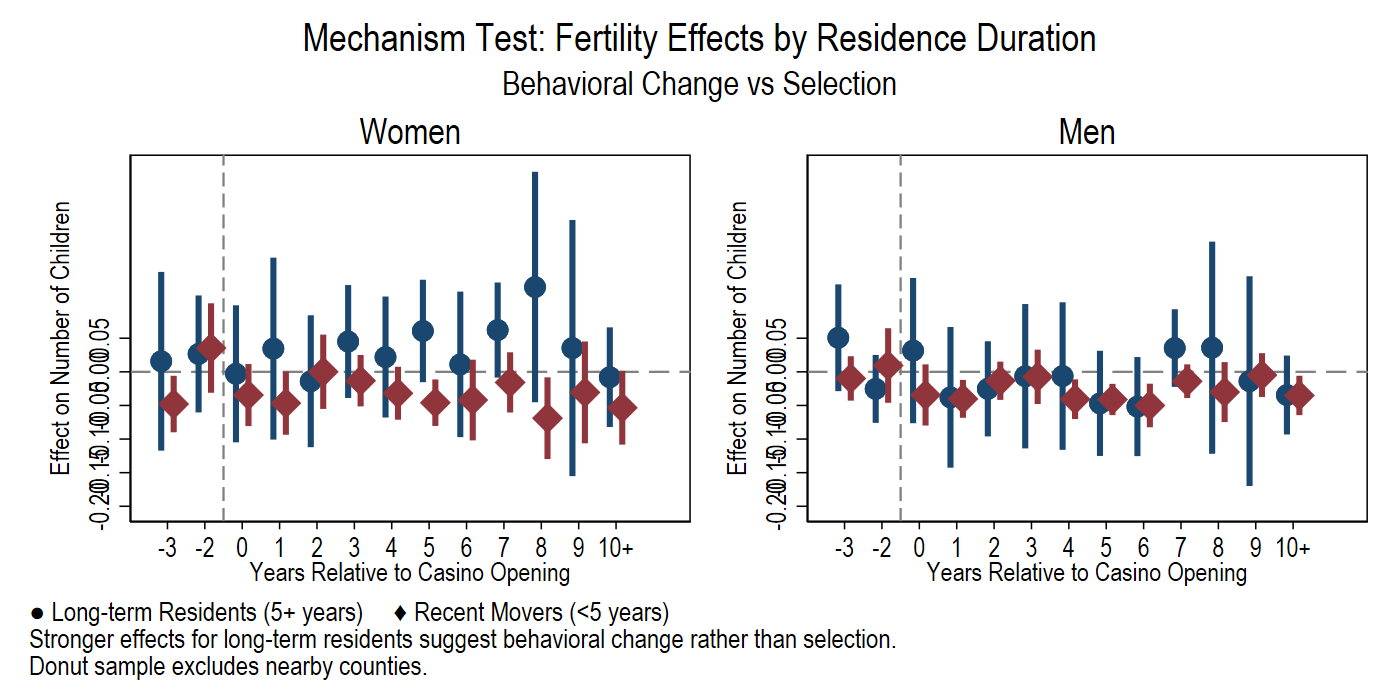
\includegraphics[width=\textwidth]{figure3_mechanism_test.png}
\caption{Mechanism Test: Fertility Effects by Residence Duration}
\label{fig:mechanism}
\end{figure}


To further validate our interpretation, Table \ref{tab:composition} 

% Table 5: Population Composition Tests - Input directly without wrapper
\begin{table}[htbp]\centering
\def\sym#1{\ifmmode^{#1}\else\(^{#1}\)\fi}
\caption{Population Composition Tests}
\begin{tabular}{l*{2}{c}}
\hline\hline
            &\multicolumn{1}{c}{(1)}&\multicolumn{1}{c}{(2)}\\
            &\multicolumn{1}{c}{Log Long-term Population}&\multicolumn{1}{c}{Long-term Population Share}\\
\hline
-3          &      -0.039         &      -0.005         \\
            &     (0.041)         &     (0.007)         \\
[1em]
-2          &       0.009         &       0.004         \\
            &     (0.045)         &     (0.009)         \\
[1em]
0           &      -0.023         &      -0.005         \\
            &     (0.036)         &     (0.006)         \\
[1em]
1           &      -0.047         &      -0.007\sym{*}  \\
            &     (0.030)         &     (0.004)         \\
[1em]
2           &      -0.015         &       0.000         \\
            &     (0.030)         &     (0.005)         \\
[1em]
3           &       0.003         &       0.000         \\
            &     (0.033)         &     (0.006)         \\
[1em]
4           &      -0.010         &      -0.000         \\
            &     (0.034)         &     (0.006)         \\
[1em]
5           &      -0.075\sym{*}  &      -0.013\sym{*}  \\
            &     (0.040)         &     (0.007)         \\
[1em]
6           &       0.005         &       0.001         \\
            &     (0.035)         &     (0.006)         \\
[1em]
7           &      -0.063         &      -0.008         \\
            &     (0.048)         &     (0.008)         \\
[1em]
8+          &      -0.038         &      -0.005         \\
            &     (0.035)         &     (0.006)         \\
\hline
Observations&       7,262         &       7,262         \\
R-squared   &       0.970         &       0.598         \\
\hline\hline
\multicolumn{3}{l}{\footnotesize Standard errors in parentheses}\\
\multicolumn{3}{l}{\footnotesize Standard errors clustered at county level in parentheses.}\\
\multicolumn{3}{l}{\footnotesize Tests whether casinos affect size/composition of long-term resident population.}\\
\multicolumn{3}{l}{\footnotesize Long-term = 5+ years in residence. Donut sample excludes nearby counties.}\\
\multicolumn{3}{l}{\footnotesize \sym{*} \(p<0.10\), \sym{**} \(p<0.05\), \sym{***} \(p<0.01\)}\\
\end{tabular}
\end{table}



\subsection{School Effects}

Table \ref{tab:schools} 

% Table 6: School Population and Enrollment Effects - Input directly without wrapper
\begin{table}[htbp]\centering
\def\sym#1{\ifmmode^{#1}\else\(^{#1}\)\fi}
\caption{School Population and Enrollment Effects}
\begin{tabular}{l*{3}{c}}
\hline\hline
            &\multicolumn{1}{c}{(1)}&\multicolumn{1}{c}{(2)}&\multicolumn{1}{c}{(3)}\\
            &\multicolumn{1}{c}{School-Age Pop}&\multicolumn{1}{c}{Total Enrollment}&\multicolumn{1}{c}{Public Enrollment}\\
\hline
t-3         &      -0.054\sym{***}&      -0.052\sym{**} &      -0.043\sym{**} \\
            &     (0.020)         &     (0.021)         &     (0.020)         \\
[1em]
t-2         &      -0.007         &      -0.004         &       0.007         \\
            &     (0.013)         &     (0.014)         &     (0.013)         \\
[1em]
t           &      -0.029\sym{*}  &      -0.025\sym{*}  &      -0.026\sym{*}  \\
            &     (0.015)         &     (0.015)         &     (0.015)         \\
[1em]
t+1         &      -0.032\sym{**} &      -0.026\sym{*}  &      -0.017         \\
            &     (0.015)         &     (0.016)         &     (0.015)         \\
[1em]
t+2         &      -0.044\sym{***}&      -0.042\sym{**} &      -0.031\sym{*}  \\
            &     (0.017)         &     (0.017)         &     (0.018)         \\
[1em]
t+3         &      -0.053\sym{***}&      -0.050\sym{***}&      -0.037\sym{**} \\
            &     (0.018)         &     (0.019)         &     (0.019)         \\
[1em]
t+4         &      -0.056\sym{***}&      -0.057\sym{***}&      -0.033         \\
            &     (0.020)         &     (0.020)         &     (0.021)         \\
[1em]
t+5         &      -0.063\sym{***}&      -0.063\sym{***}&      -0.046\sym{**} \\
            &     (0.020)         &     (0.020)         &     (0.022)         \\
[1em]
t+6         &      -0.069\sym{***}&      -0.065\sym{***}&      -0.041\sym{*}  \\
            &     (0.022)         &     (0.022)         &     (0.022)         \\
[1em]
t+7         &      -0.078\sym{***}&      -0.075\sym{***}&      -0.064\sym{***}\\
            &     (0.022)         &     (0.023)         &     (0.024)         \\
[1em]
t+8+        &      -0.064\sym{**} &      -0.063\sym{**} &      -0.042         \\
            &     (0.027)         &     (0.027)         &     (0.026)         \\
\hline
Observations&       7,580         &       7,580         &       7,580         \\
R-squared   &       0.991         &       0.991         &       0.990         \\
\hline\hline
\multicolumn{4}{l}{\footnotesize Standard errors in parentheses}\\
\multicolumn{4}{l}{\footnotesize Standard errors clustered at county level in parentheses.}\\
\multicolumn{4}{l}{\footnotesize All variables in logs. School-age = 5-17 years.}\\
\multicolumn{4}{l}{\footnotesize Donut sample excludes nearby counties. *** p<0.01, ** p<0.05, * p<0.1.}\\
\multicolumn{4}{l}{\footnotesize \sym{*} \(p<0.10\), \sym{**} \(p<0.05\), \sym{***} \(p<0.01\)}\\
\end{tabular}
\end{table}


\subsection{Religious Effects}

Table \ref{tab:religious} examines effects on religious adherence using four specifications. Our preferred specification with state-year fixed effects reveals a 9.5\% decline in religious adherence, suggesting casinos weaken an important family-supporting institution.

% Table 7: Religious Adherence Effects - Input directly without wrapper
\begin{table}[h]\centering
\def\sym#1{\ifmmode^{#1}\else\(^{#1}\)\fi}
\caption{Religious Adherence Effects}
\begin{tabular}{l*{4}{c}}
\hline\hline
            &\multicolumn{1}{c}{(1)}&\multicolumn{1}{c}{(2)}&\multicolumn{1}{c}{(3)}&\multicolumn{1}{c}{(4)}\\
            &\multicolumn{1}{c}{Baseline}&\multicolumn{1}{c}{Medium Religious}&\multicolumn{1}{c}{State-Year FE}&\multicolumn{1}{c}{Differenced}\\
\hline
post\_treatment&     -11.952         &     -37.364\sym{***}&     -34.850\sym{**} &                     \\
            &    (17.322)         &    (11.626)         &    (15.172)         &                     \\
\hline
Observations&       9,418         &       3,139         &       9,415         &       6,275         \\
R-squared   &       0.932         &       0.975         &       0.960         &       0.826         \\
\hline\hline
\multicolumn{5}{l}{\footnotesize Standard errors in parentheses}\\
\multicolumn{5}{l}{\footnotesize Standard errors clustered at county level in parentheses.}\\
\multicolumn{5}{l}{\footnotesize Dependent variable: religious adherents per 1,000 population.}\\
\multicolumn{5}{l}{\footnotesize Medium Religious = counties in middle tercile of 2000 adherence.}\\
\multicolumn{5}{l}{\footnotesize State-Year FE preferred specification. *** p<0.01, ** p<0.05, * p<0.1.}\\
\multicolumn{5}{l}{\footnotesize \sym{*} \(p<0.10\), \sym{**} \(p<0.05\), \sym{***} \(p<0.01\)}\\
\end{tabular}
\end{table}


\begin{figure}[H]
\centering
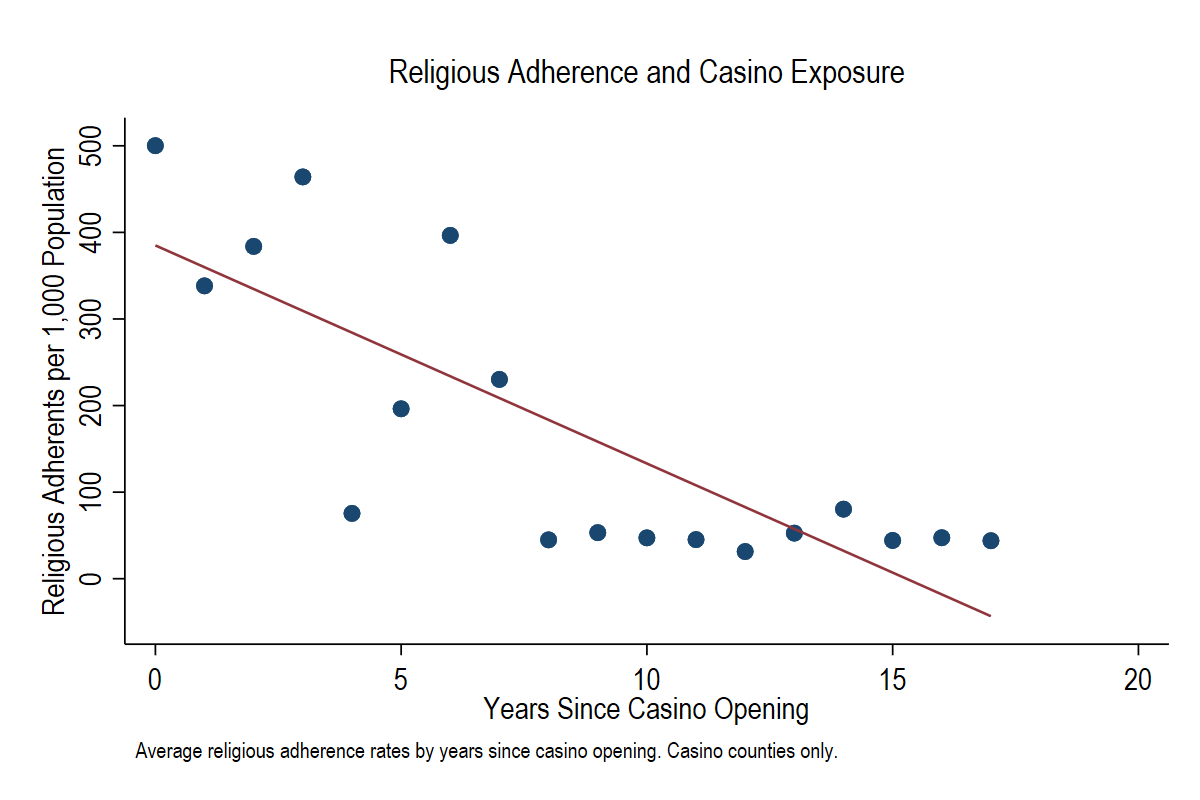
\includegraphics[width=\textwidth]{figure4_religious_exposure.png}
\caption{Mechanism Test: religious exposure}
\label{fig:relig}
\end{figure}

Table \ref{tab:denominations} 

% Table 8: Religious Effects by Denomination - Input directly without wrapper
\begin{table}[htbp]\centering
\def\sym#1{\ifmmode^{#1}\else\(^{#1}\)\fi}
\caption{Religious Effects by Denomination}
\begin{tabular}{l*{8}{c}}
\hline\hline
            &\multicolumn{2}{c}{Catholic}               &\multicolumn{2}{c}{Evangelical}            &\multicolumn{2}{c}{Mainline}               &\multicolumn{2}{c}{Southern Baptist}       \\\cmidrule(lr){2-3}\cmidrule(lr){4-5}\cmidrule(lr){6-7}\cmidrule(lr){8-9}
            &\multicolumn{1}{c}{(1)}&\multicolumn{1}{c}{(2)}&\multicolumn{1}{c}{(3)}&\multicolumn{1}{c}{(4)}&\multicolumn{1}{c}{(5)}&\multicolumn{1}{c}{(6)}&\multicolumn{1}{c}{(7)}&\multicolumn{1}{c}{(8)}\\
            &\multicolumn{1}{c}{Baseline}&\multicolumn{1}{c}{State-Yr FE}&\multicolumn{1}{c}{Baseline}&\multicolumn{1}{c}{State-Yr FE}&\multicolumn{1}{c}{Baseline}&\multicolumn{1}{c}{State-Yr FE}&\multicolumn{1}{c}{Baseline}&\multicolumn{1}{c}{State-Yr FE}\\
\hline
post\_treatment&     -73.206\sym{***}&     -59.441\sym{***}&      52.966\sym{***}&      18.803\sym{***}&      24.650\sym{***}&      13.144\sym{***}&      42.734\sym{***}&       6.000\sym{***}\\
            &    (25.604)         &    (13.058)         &     (7.542)         &     (4.447)         &     (6.110)         &     (3.816)         &     (5.320)         &     (2.224)         \\
\hline
Observations&       9,232         &       9,229         &       9,398         &       9,395         &       9,387         &       9,384         &       8,105         &       8,102         \\
R-squared   &       0.811         &       0.922         &       0.796         &       0.926         &       0.811         &       0.917         &       0.742         &       0.914         \\
\hline\hline
\multicolumn{9}{l}{\footnotesize Standard errors in parentheses}\\
\multicolumn{9}{l}{\footnotesize Standard errors clustered at county level in parentheses.}\\
\multicolumn{9}{l}{\footnotesize Dependent variables: denomination adherents per 1,000 population.}\\
\multicolumn{9}{l}{\footnotesize Baseline = county + year FE. State-Yr FE = county + state-year FE.}\\
\multicolumn{9}{l}{\footnotesize *** p<0.01, ** p<0.05, * p<0.1.}\\
\multicolumn{9}{l}{\footnotesize \sym{*} \(p<0.10\), \sym{**} \(p<0.05\), \sym{***} \(p<0.01\)}\\
\end{tabular}
\end{table}



Figure \ref{fig:religious} shows the relationship between religious adherence and years since casino opening, revealing a clear negative correlation consistent with our regression results.

\begin{figure}[H]
\centering
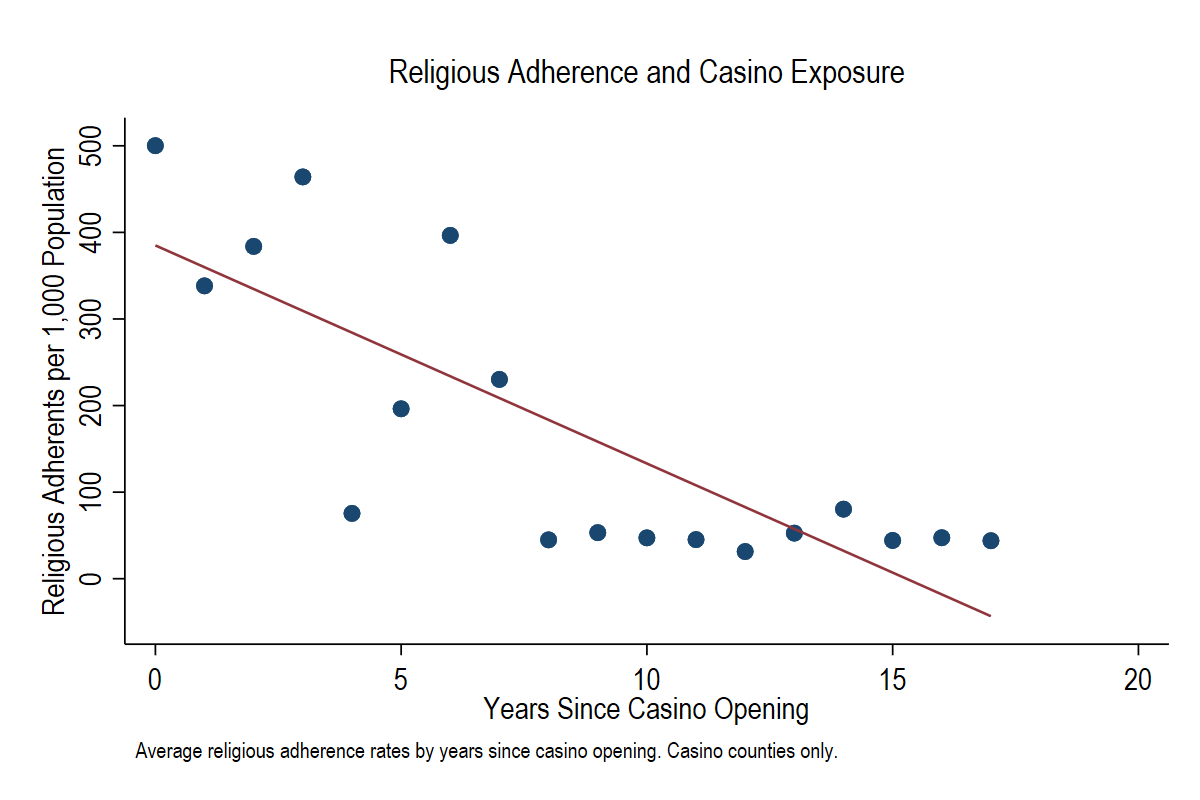
\includegraphics[width=0.8\textwidth]{figure4_religious_exposure.png}
\caption{Religious Adherence and Casino Exposure}
\label{fig:religious}
\end{figure}

\section{Robustness: Spillover Effects}

Table \ref{tab:spillover} 

% Table 9: Spillover Effects - Input directly without wrapper
\begin{table}[htbp]\centering
\def\sym#1{\ifmmode^{#1}\else\(^{#1}\)\fi}
\caption{Spillover Effects: Casino vs Nearby Counties}
\begin{tabular}{l*{4}{c}}
\hline\hline
            &\multicolumn{1}{c}{(1)}&\multicolumn{1}{c}{(2)}&\multicolumn{1}{c}{(3)}&\multicolumn{1}{c}{(4)}\\
            &\multicolumn{1}{c}{Fertility (W)}&\multicolumn{1}{c}{Fertility (M)}&\multicolumn{1}{c}{Child Pop}&\multicolumn{1}{c}{Religious}\\
\hline
Casino County × Post&     -0.0550\sym{***}&     -0.0299\sym{***}&     -0.0258\sym{**} &    -16.3704         \\
            &    (0.0186)         &    (0.0085)         &    (0.0122)         &   (16.3914)         \\
[1em]
Nearby County × Post&      0.0000         &      0.0000         &      0.0000         &      0.0000         \\
            &         (.)         &         (.)         &         (.)         &         (.)         \\
\hline
Observations&   8,995,331         &   9,080,818         &       9,160         &       9,418         \\
R-squared   &       0.242         &       0.206         &       0.992         &       0.932         \\
\hline\hline
\multicolumn{5}{l}{\footnotesize Standard errors in parentheses}\\
\multicolumn{5}{l}{\footnotesize Standard errors clustered at county level in parentheses.}\\
\multicolumn{5}{l}{\footnotesize Tests for spillover effects to nearby counties. Justifies donut design.}\\
\multicolumn{5}{l}{\footnotesize Reference group: control counties. *** p<0.01, ** p<0.05, * p<0.1.}\\
\multicolumn{5}{l}{\footnotesize \sym{*} \(p<0.10\), \sym{**} \(p<0.05\), \sym{***} \(p<0.01\)}\\
\end{tabular}
\end{table}



\end{document}